\problemname{Matrix Keypad}

\illustration{0.3}{keypad.png} 

%
% https://openclipart.org/detail/217230/code-alarm-keypad
% public domain


A matrix keypad consists of an $r \times c$ grid of buttons.
Additionally, there is one wire for each row and one wire for each
column.  These wires are exposed through pins so the keypad can be
connected to a larger circuit.

When a button at row $i$ and column $j$ is pressed, the wire for row
$i$ and the wire for column $j$ will carry an electrical current.  If
just a single button is pressed, it can be identified by sequentially
checking if a current can be detected at each row wire and at each
column wire.

Unfortunately, when multiple buttons are pressed at the same time, it
may not be possible to uniquely identify which buttons are pressed.
The only information you can have is this: for each wire, whether
there is at least one button along that wire being pressed.

%\begin{center}
%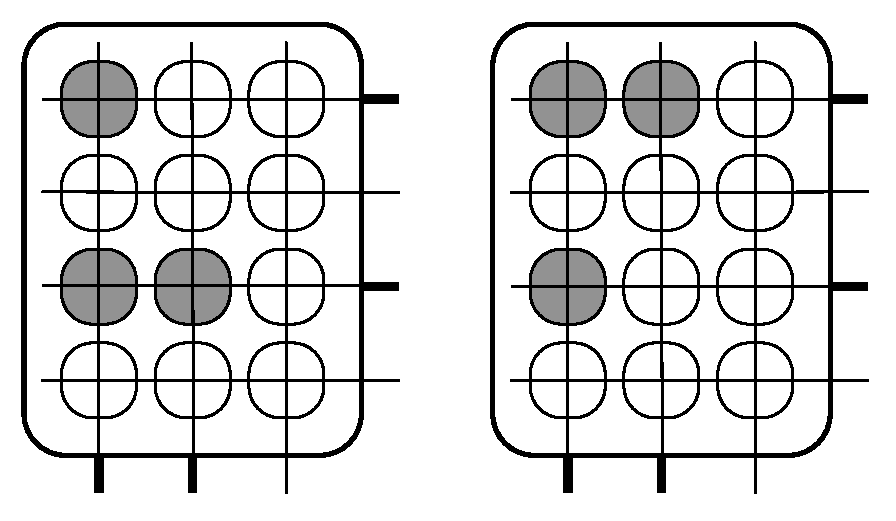
\includegraphics[scale=0.8]{keypad.pdf}
%\end{center}

The software you are using to detect which buttons are pressed was
poorly implemented.  After probing the keypad, it stores the
information in an $r \times c$ grid of \texttt{0/1} values. The value
stored in row $i$ and column $j$ of this grid is \texttt{1} if there
is at least one button in row $i$ and at least one (possibly
different) button in column $j$ that is pressed.  Otherwise, the value
that is stored at this position is \texttt{0}.

Your job is to interpret as much information from such a grid as possible.
Determine which buttons are definitely pressed and which buttons are definitely
not pressed.

\section*{Input}
The first line of input contains a single positive integer $T \leq 200$ indicating
the number of test cases. The first line of each test case
contains two integers $r$ and $c$ where $1 \leq r \leq 10$
and $1 \leq c \leq 10$. This indicates that the keypad is an $r \times c$
grid of buttons.

The remaining $r$ lines of a test case describe the grid. The $i$th row
contains a string of consecutive \texttt{0} and
\texttt{1} characters. These will not be separated by spaces.

\section*{Output}
For each test case, output the following. If there is no combination of
button presses on the keypad that would produce this \texttt{0}/\texttt{1}
grid then simply output a line containing the word \texttt{impossible}

Otherwise, you should output $r$ lines, each containing a string of length
$c$. This should describe a grid where the character at row $i$ and column
$j$ is:
\begin{itemize}
\item \texttt{N} if no button combination that produces
the input grid has the $j$th button on row $i$ being pressed.
\item \texttt{P} if all button combinations that produce
the input grid have the $j$th button on row $i$ being pressed.
\item \texttt{I} if some, but not all,
button combinations that produce the input
grid have the $j$th button on row $i$ being pressed.
\end{itemize}

Finally, the last line of each test case should be followed
by the string \verb|----------| (10 dashes).
